\begin{task}{441}
Перечислите все попарно неизоморфные связные простые графы на \(8\) вершинах, в которых ровно три блока и при этом не более двух простых циклов. Подробно описывать перебор не нужно (не нужно описывать получение каждого отдельного графа), но обязательно стоит разделить графы на группы по значениям параметров, по которым осуществлялся перебор (параметров должно быть минимум два, второй из которых позволяет перебирать графы с одинаковым значением первого параметра). При переборе случаев используйте вложенные окружения \textbf{enumerate} и окружение \textbf{figure}, не забудьте также использовать пары команд \textbf{ref} и \textbf{label} для описания рисунков. Описание случаев перебора должно происходить в тексте решения в tex-файле, а не внутри рисунков!. 
\end{task}
\begin{solution}
Разделим графы на группы по количеству простых циклов: ноль циклов, один цикл и два цикла.
\begin{enumerate}

\item Если в связном графе нет простых циклов, то это дерево. В дереве на восьми вершинах семь рёбер. Каждое ребро дерева это отдельный блок. Значит, графы без простых циклов под условие не подходят.

\item 
Если в связном графе один цикл, то на этом цикле либо одна, либо две точки сочленения.
\begin{enumerate}

\item 
Если в графе только одна точка сочленения попадает на цикл, то таких графов только два. Они изображены на рис.~\ref{fig:441:0000}.

\begin{figure}[H]
    \centering
    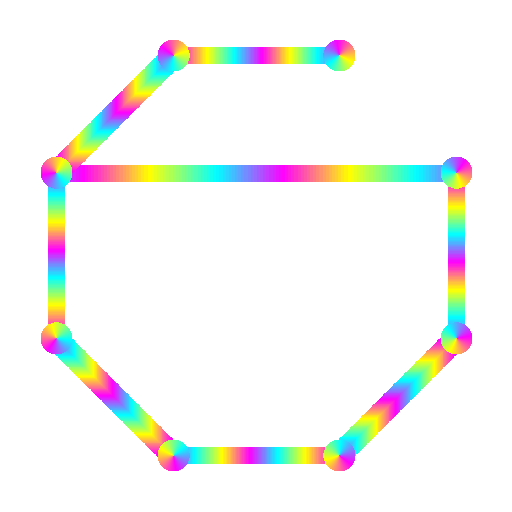
\includegraphics[width=4cm, keepaspectratio]{Fall/img/test441-0000.png}
    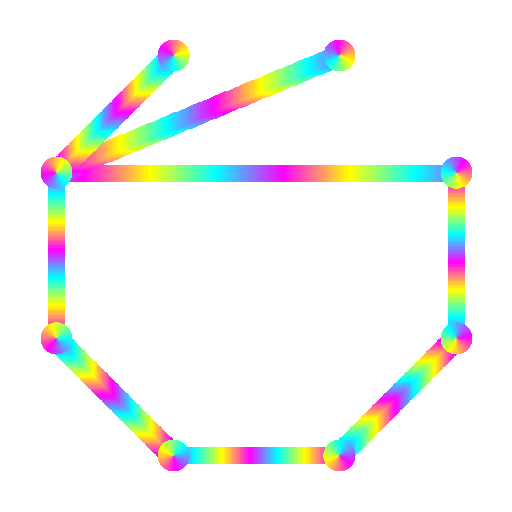
\includegraphics[width=4cm, keepaspectratio]{Fall/img/test441-0001.png}
    \caption{Графы, в которых только одна точка сочленения попадает на цикл.}
    \label{fig:441:0000}
\end{figure}

\item 
Если в графе две точки сочленения попадают на цикл, то переберём графы по возрастанию расстояния между ними. Полученные графы изображены на рис.~\ref{fig:441:0002}.

\begin{figure}[H]
    \centering
    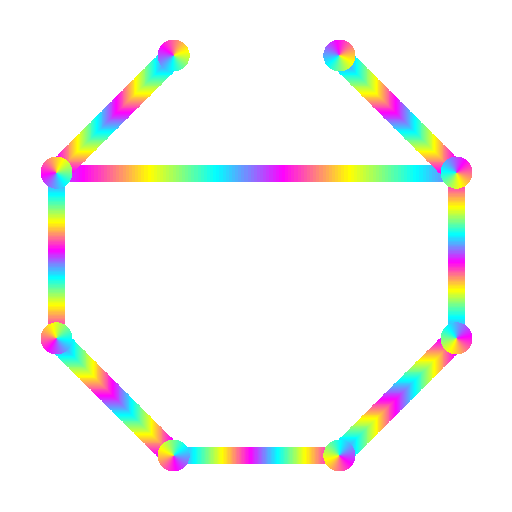
\includegraphics[width=4cm, keepaspectratio]{Fall/img/test441-0002.png}
    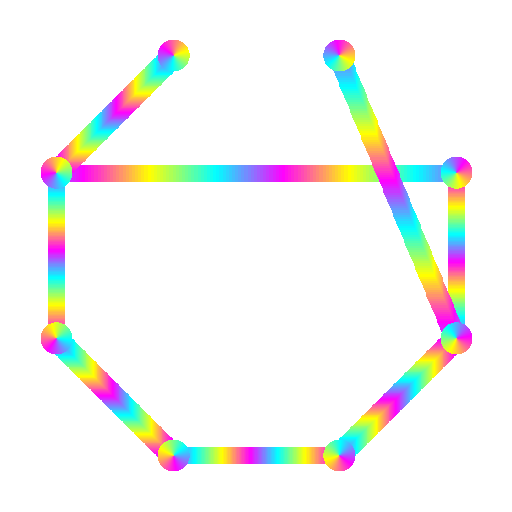
\includegraphics[width=4cm, keepaspectratio]{Fall/img/test441-0003.png}
    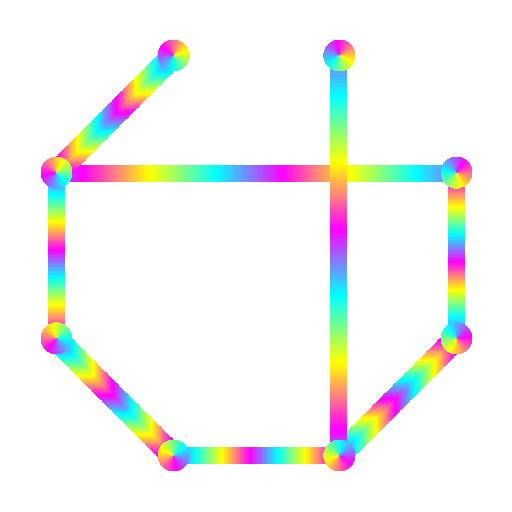
\includegraphics[width=4cm, keepaspectratio]{Fall/img/test441-0004.png}
    \caption{Графы, в которых две точки сочленения попадают на цикл.}
    \label{fig:441:0002}
\end{figure}

\end{enumerate}

\item 
Если в связном графе два цикла, то они либо имеют общую вершину, либо соединены ребром.
\begin{enumerate}

\item 
Если циклы не имеют общей вершины, то переберём их по длине минимального цикла. Получим графы, изображённые на рис.~\ref{fig:441:0005}.

\begin{figure}[H]
    \centering
    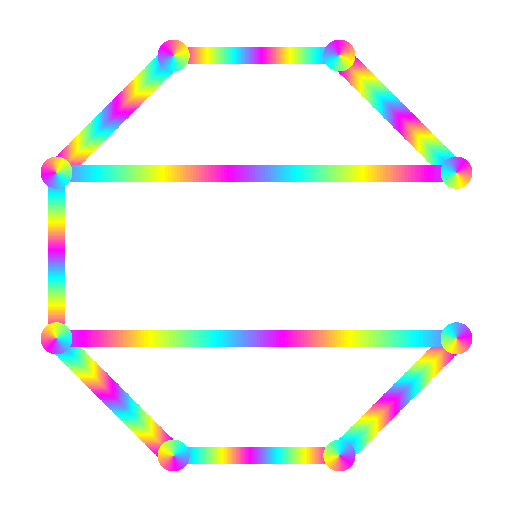
\includegraphics[width=4cm, keepaspectratio]{Fall/img/test441-0005.png}
    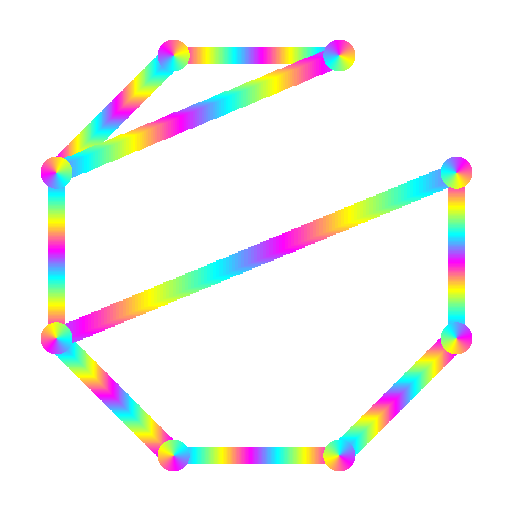
\includegraphics[width=4cm, keepaspectratio]{Fall/img/test441-0006.png}
    \caption{Графы с двумя циклами, которые соединены ребром.}
    \label{fig:441:0005}
\end{figure}

\item 
Если циклы имеют общую вершину, то в графе есть висячая вершина. Переберём графы по длине минимального цикла, потом по расстоянию от места присоединения этой вершины до общей вершины циклов. Получим графы, изображённые на рис.~\ref{fig:441:0007}.

\begin{figure}[H]
    \centering
    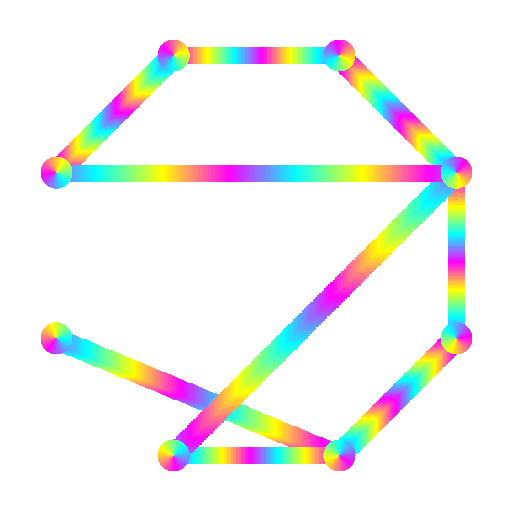
\includegraphics[width=4cm, keepaspectratio]{Fall/img/test441-0007.png}
    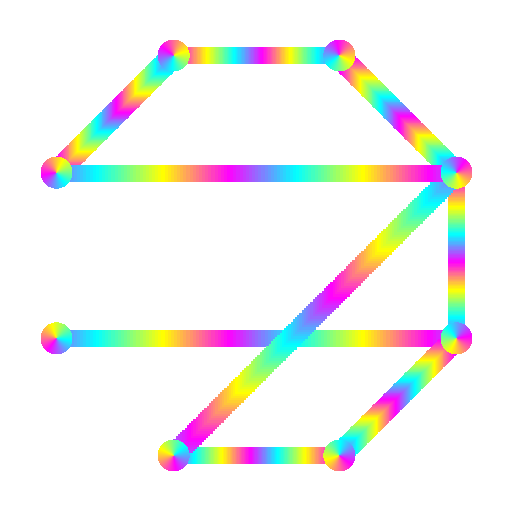
\includegraphics[width=4cm, keepaspectratio]{Fall/img/test441-0008.png}
    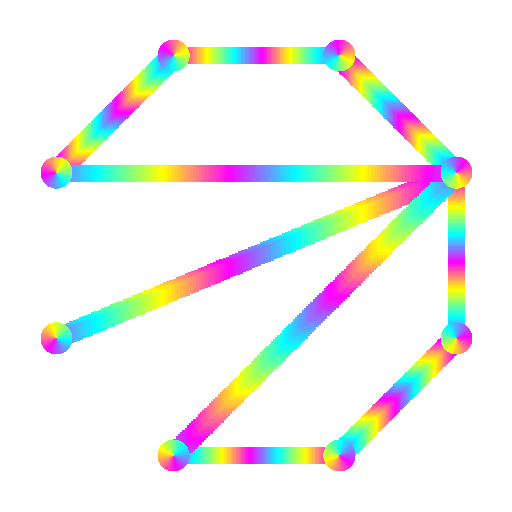
\includegraphics[width=4cm, keepaspectratio]{Fall/img/test441-0009.png}
    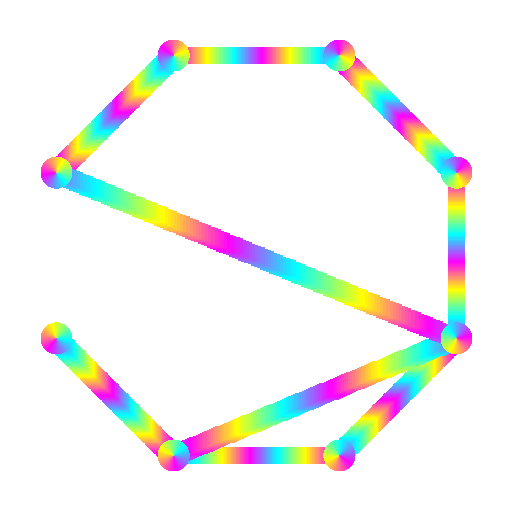
\includegraphics[width=4cm, keepaspectratio]{Fall/img/test441-0010.png}
    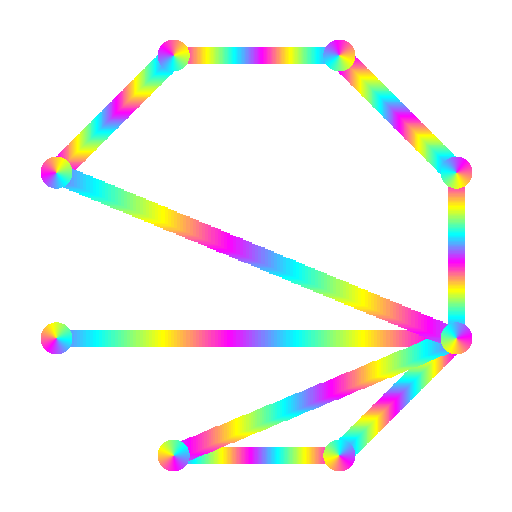
\includegraphics[width=4cm, keepaspectratio]{Fall/img/test441-0011.png}
    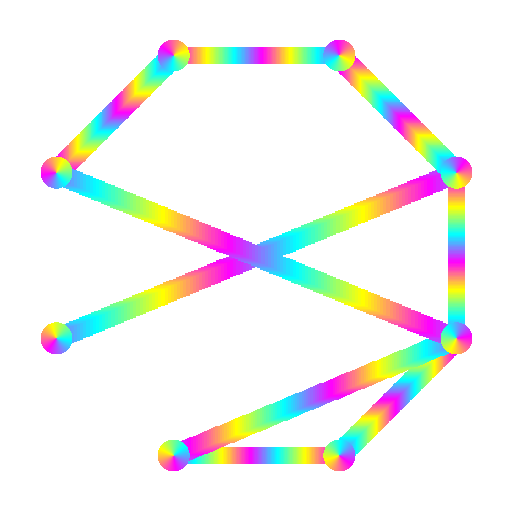
\includegraphics[width=4cm, keepaspectratio]{Fall/img/test441-0012.png}
    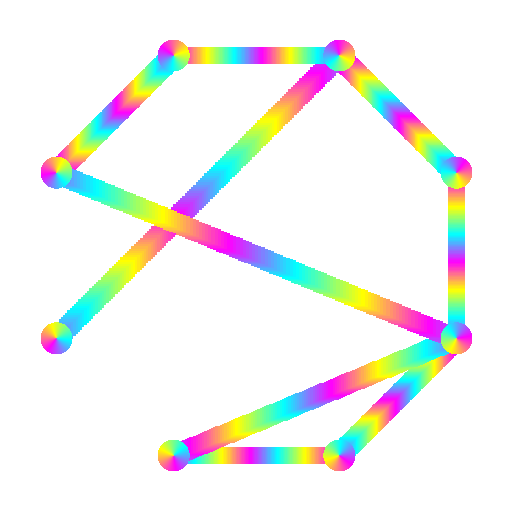
\includegraphics[width=4cm, keepaspectratio]{Fall/img/test441-0013.png}
    \caption{Графы с двумя циклами, которые имеют общую вершину.}
    \label{fig:441:0007}
\end{figure}


\end{enumerate}
\end{enumerate}
Все графы, подходящие под условие перечислены.

\end{solution}
